% Results and discussion: measured latency, throughput and utilization of the accelerator (issue #71).
% Numbers come from results/phase2/cycle_counts.csv and results/phase2/tiled_cycles.csv,
% which tb_systolic_top writes (#69), and the figure from model/perf_model.py (#73).
% Throughput per second uses the maximum clock frequency in results/phase2/synth/synth_summary.csv (#75).
% The waveform captures are in results/phase2/waveforms/ (#66).

\subsection{Latency, Throughput and Utilization}
\textbf{Single runs.} The end-to-end testbench drove all 112 cases of the $K \neq N$ vector set through the host ports, with $k_{\mathrm{len}}$ from 1 to 16 and random filler stored past $k_{\mathrm{len}}$ in both operand buffers. Every element of $C$ matched the golden model, so no element past $k_{\mathrm{len}}$ ever reached the array. Every run was busy for exactly $k_{\mathrm{len}} + 2N$ cycles, from 9 for $k_{\mathrm{len}} = 1$ to 24 for $k_{\mathrm{len}} = 16$, and $k_{\mathrm{len}} + 2N - 2$ of them were compute steps, as the timing contract requires. A run performs $N^2 k_{\mathrm{len}}$ multiply-accumulates, so the array completes $N^2 k_{\mathrm{len}} / (k_{\mathrm{len}} + 2N)$ of them per busy cycle: 5.3 for $k_{\mathrm{len}} = 4$ and 10.7 for $k_{\mathrm{len}} = 16$, against a peak of $N^2 = 16$. At the array's maximum clock frequency after place and route, 56.83~MHz, that is 303 million multiply-accumulates per second for $k_{\mathrm{len}} = 4$ and 606 million for $k_{\mathrm{len}} = 16$, against a peak of 909 million. The capture \path{results/phase2/waveforms/systolic_top_klen.png} shows one such run, with $k_{\mathrm{len}} = 5$, cycle by cycle.

\textbf{Utilization.} Each PE adds $k_{\mathrm{len}}$ products during the $k_{\mathrm{len}} + 2N - 2$ compute steps, so the fraction of PE-cycles doing useful work is $k_{\mathrm{len}} / (k_{\mathrm{len}} + 2N - 2)$. Fig.~\ref{fig:util} shows it for three array sizes. On the $4 \times 4$ array it rises from 14.3\,\% for $k_{\mathrm{len}} = 1$ to 40\,\% for $k_{\mathrm{len}} = 4$ and 72.7\,\% for $k_{\mathrm{len}} = K_{\max} = 16$, and every measured run lies on that curve. Beyond $K_{\max}$ a product needs a second chunk, which pays the fill and drain again: utilization falls to 58.6\,\% at $K = 17$, where the second chunk has length 1, and then climbs again. A larger array needs longer runs to reach the same utilization, because its fill and drain take $2N - 2$ steps.

\begin{figure}[t]
\centering
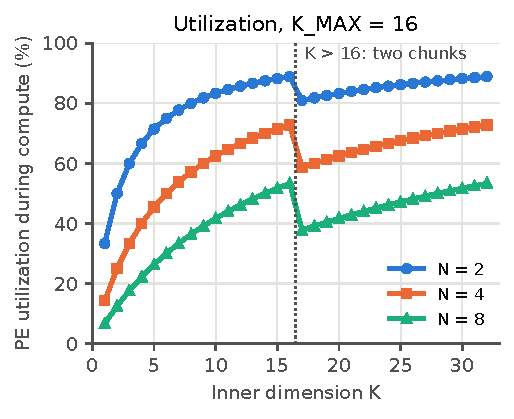
\includegraphics[width=0.9\columnwidth]{utilization_vs_k}
\caption{PE utilization during compute, $K / \sum (k_{\mathrm{len}} + 2N - 2)$ over a product's chunks, against the inner dimension $K$ for $K_{\max} = 16$. Products with $K > 16$ run as two chunks.}
\label{fig:util}
\end{figure}

\textbf{Tiled products.} The same testbench multiplied all 26 products of the tiled vector set, from $1 \times 1 \times 1$ to $9 \times 33 \times 7$ and $4 \times 64 \times 4$, by cutting them into tiles and chunks through the host ports as Section~III-E describes. Every element of every product matched the golden result, including the $4 \times 64 \times 4$ product of $-128$ values, whose elements reach 1,048,576 across four accumulate runs. The capture \path{results/phase2/waveforms/systolic_top_accumulate.png} shows the second and third chunks of the $4 \times 40 \times 4$ product starting without a clear cycle and adding onto the partial sums. Table~\ref{tab:tiled} lists the six directed products. On every product the busy cycles equal~\eqref{eq:tilebusy} summed over the tiles, and the total cycles of the host procedure, with one element loaded and read per cycle, equal the count of Section~III-E: $NK$ cycles of loading, one start pulse per run and $N^2$ cycles of readout per tile, on top of the busy cycles.

\begin{table}[t]
\centering
\caption{Measured cycles of the directed tiled products ($N = 4$, $K_{\max} = 16$)}
\label{tab:tiled}
\footnotesize
\setlength{\tabcolsep}{2.6pt}
\begin{tabular}{@{}lccrrrr@{}}
\toprule
Product & $M{\times}K{\times}P$ & Tiles, chunks & Busy & Total & Busy/total & Util. \\
\midrule
exact & $8{\times}8{\times}8$ & 4, 1 & 64 & 260 & 24.6\,\% & 50.0\,\% \\
pad\_all & $5{\times}7{\times}6$ & 4, 1 & 60 & 240 & 25.0\,\% & 21.9\,\% \\
chunks & $4{\times}40{\times}4$ & 1, 3 & 62 & 241 & 25.7\,\% & 64.5\,\% \\
pad\_chunks & $9{\times}33{\times}7$ & 6, 3 & 330 & 1236 & 26.7\,\% & 39.4\,\% \\
single & $1{\times}1{\times}1$ & 1, 1 & 9 & 30 & 30.0\,\% & 0.7\,\% \\
max\_neg.\_long & $4{\times}64{\times}4$ & 1, 4 & 93 & 369 & 25.2\,\% & 68.8\,\% \\
\bottomrule
\end{tabular}

\smallskip
\raggedright
Total counts loading, start pulses, busy cycles and readout. Util.\ is $MKP / (N^2 \cdot \mathrm{busy})$: useful multiply-accumulates over what the array could do while busy.
\end{table}

Two costs stand out. First, the array is busy for only 22.9 to 30.0\,\% of the host procedure across the 26 products: loading a run's operands one element per cycle takes $N k_{\mathrm{len}}$ cycles, longer than the run's $k_{\mathrm{len}} + 2N$ busy cycles for every $k_{\mathrm{len}} \ge 3$, and each tile adds $N^2$ cycles of readout. Second, zero padding costs as much time as real work. The $5 \times 7 \times 6$ product keeps the array busy almost as long as the $8 \times 8 \times 8$ one, 60 cycles against 64, but does fewer than half as many useful multiply-accumulates, so its utilization is 21.9\,\% against 50.0\,\%. Long inner dimensions use the array best: the single-tile products with three and four chunks reach 64.5 and 68.8\,\%. Counted end to end at 56.83~MHz, the 26 products complete 1.9 to 158 million multiply-accumulates per second: 112 million for the $8 \times 8 \times 8$ product, against 455 million during its busy cycles alone.
